\chapter{Robot Design}
\label{chap:mech_design}

The final design of the hopping robot is described in this chapter. We first look at two previous designs devised to make use of SLOM effect. After ironing out some deficiencies, we arrive at a simplistic design that satisfies our criteria.
\begin{figure}[H]
\centering
\subfloat[Design 1]{\label{fig:3_design1} 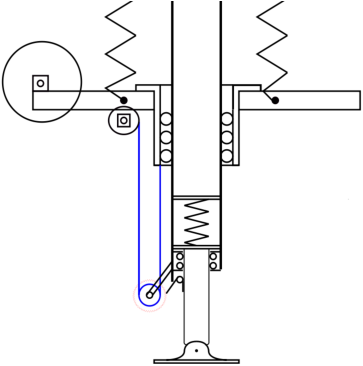
\includegraphics[width=0.5\textwidth]{fig/design1.pdf}}
\subfloat[Design 2]{\label{fig:3_design2} 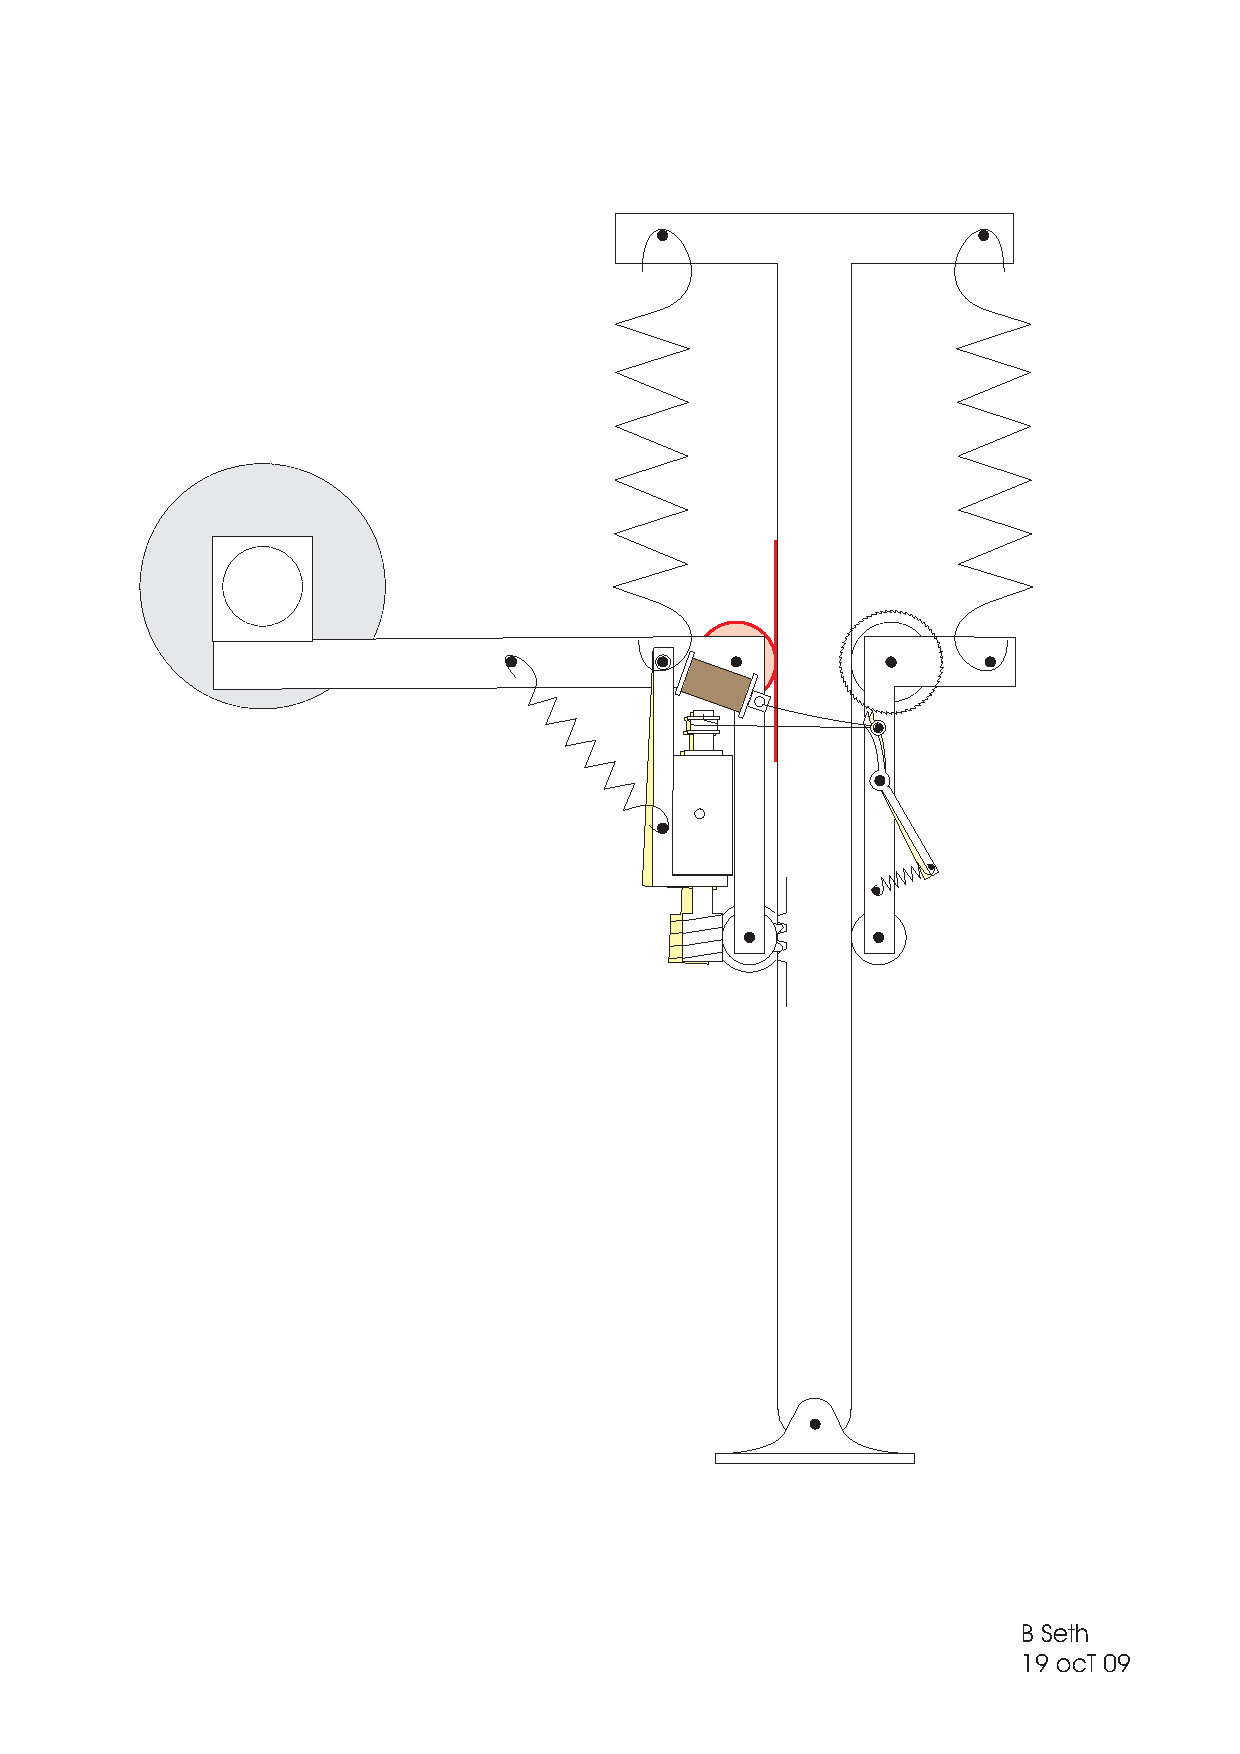
\includegraphics[width=0.5\textwidth]{fig/design2.pdf}}
\caption{Previous hopping robot designs : Approx. height = $500\;mm$}
\label{fig:3_prevdes}
\end{figure}

\section{Mechanical}
\subsection*{Previous Designs}
\label{sec_3:mechanical}

A description of the two designs is given in the report for Stage I \cite{stage1}. The evaluation 
of these two designs is as follows,
\subsubsection*{Design 1}
\begin{enumerate}
  \item
  It has to be ensured that the winding winch does not slip over the pulley when the platform is suddenly released from the constraint. At the same time, the winch must be free enough so as not to hinder the 	movement of the platform after the release.
  \item
  The platform moves over the leg with the help of a circular bushing. There is another bushing for the lower leg to move into the upper leg. These circular bushings are light and durable.
  \item
  The hatch that is a crucial part of the energy release and the constraint mechanism is the weakest part, but it can break easily.
\end{enumerate}

\subsubsection*{Design 2}
\begin{enumerate}
 \item
The sleeve of the motor is kept on the same side as that of the reaction wheel and helps to provide an offset mass for the SLOM effect. Body mass also helps to obtain an offset C.G.; thus the distance of the reaction wheel from the axis need not as be as large as calculated in the adjoining analysis.
\item
The worm-worm wheel on the rack mechanism provides a huge mechanical advantage and thus reduces the maximum torque required from the motor. This scales down the mechanical system as well as the electronic system requirements.
\item
All the force of the extension springs is coming as an axial load on the shaft of the motor. We thus
need to choose a gearbox that can handle these axial loads.
\item
The friction pulley has to work against the pual spring, sleeve spring and the horizontal component of the rack force ($k\:x\:tan\:\theta$) to keep the string in tension. This is compounded by the fact that the there is a maximum $\omega$ the motor can
accelerate to in the energy storing phase. It is much better if this $\omega$ is dictated by the torque requirements which are as
critical rather than this mechanism.
\item
Less resolution on the desirable extension of springs because we are operating on a rack. This can however be easily taken care of in the pitch control law.
\item
The constraint mechanism for Design 2 is not reliable enough and should be improved upon. The major problem is to provide an opposing force to the horizontal component of the rack--worm-wheel force ($k\:x\:tan\:\theta$). This force has to be present when the motor is extending the springs and should be removed before we release the ratchet so that the platform along with the motor-sleeve is free to move up. To disengage the motor from the rack, the spring shown in the left part of Fig. \ref {fig:3_design2} will have to be there as well.
\end{enumerate}

\subsection*{Final solution}
Both the designs given in Section \ref{sec_3:mechanical} had significant drawbacks and hence a newer design was made utilizing their individual mechanisms and the knowledge gained from analyses.

The salient features of this design are as follows,
\begin{enumerate}
  \item 
  As shown, in the figure, it consists of two large flanges with all the components arranged inside it. Enclosing the components inside the flanges makes it a compact, closed system with only essential components like batteries, motors, circuit boards being accessible from outside.
  \item
  One major component of this design is the rack and pinion mechanism. It is difficult to cut a 45 degree rack due to fabrication constraints. However, this mechanism has been built and fixed on the robot successfully.
  \item
  The whole robot is built in such a way that it can be pivoted fully near its C.G. to a test--rig. This test--rig simply consists of two large columns from which the robot hangs. It is a simple contraption and should prove handy while performing experiments on the robot.
  \item
  The ratchet and paul mechanism is on the same axis as the band drive. There is a servo motor on the outer side near the paul to actuate it (which is not shown here).
  \item
  Another servo motor sits on the vertical portion of the robot to ensure that the motor sleeve gets detached after extending the spring.
  \item
  We have ensured that the C.G. of the system lies along its centerline and hence there are no lateral moments. This is done by putting batteries on the opposite side of the reaction wheel motor.
\end{enumerate}

\begin{figure}[!htp]
\centering
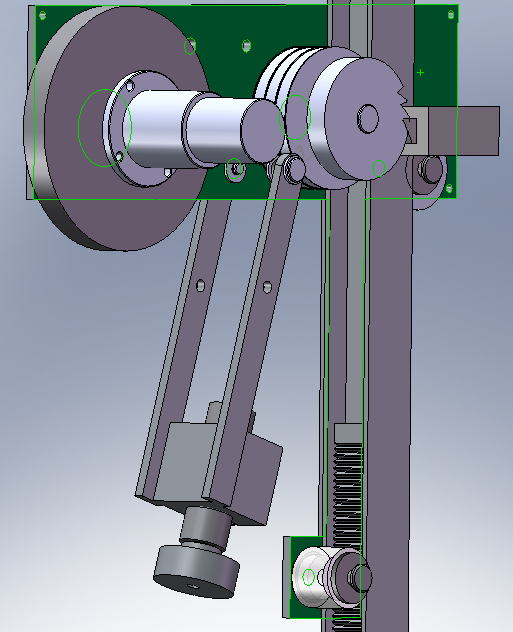
\includegraphics[scale=0.8]{fig/hopper_detach.png}
\caption[Solidworks hopping robot assembly]{Solidworks hopping robot assembly : Motor sleeve, reaction wheel and rack and pinion. Note that one of flanges is hidden in the picture to see the internal components}
\label{fig:3_solidworks1}
\end{figure}

\section{Analyses}
\label{sec_4:analyses}
We need to find approximate design estimates of the hopping robot by performing analysis. The following three values are what we are interested in.
\begin{enumerate}
\item
Masses of the platform and the leg
\item
Dimensions of the reaction wheel based on the above masses
\item
Choice of winding and reaction wheel motors
\end{enumerate}

\subsection*{$2$ mass problem}
\begin{figure}[!htp]
\centering
\begin{tikzpicture}[scale=0.45]
\draw (-3,0) -- (3,0);
\foreach \x in {-2.5,-2,...,2.5}
\draw (\x,0) -- (\x+0.5,-0.5);

\path (-2,7) coordinate(M1);
\path (2,10) coordinate(M2);
\path (-0.6,2) coordinate(m1);
\path (0.6,3.2) coordinate(m2);

\draw [thick](M1) rectangle (M2) node[midway]{\huge{$M$}};
\draw [thick](m1) rectangle (m2) node[midway]{\Large{$m$}};

\path (-2.5,0) coordinate (O);
\path (-2.5,2.6) coordinate (SPL);
\path (-2.5,8.5) coordinate (H);

\draw[<->] [semithick](O)++(-0.5,0) -- (-3,8.5) node[midway, left]{$H$};
\draw[<->] [semithick](SPL) -- (H) node[midway, right]{$l_0$};

\draw[snake=coil, segment amplitude=8pt] (0,3.2) -- (0,7) node[midway,right=2ex]{$k$};
\end{tikzpicture}
\caption[2 mass problem]{2 mass problem \cite{simit}}
\label{fig:3_2mass}
\end{figure}
The basic idea behind a hopper is like that of the 2 masses connected by a spring problem. If the system shown in Fig.
\ref{fig:3_2mass} is allowed to fall from a height, the heavier mass pulls the smaller mass with it back into the air
after impact. Every cycle is accompanied by a loss in energy due to the inelastic impact of the smaller mass with the
ground. If we pump this energy back into the system using an external agent in every cycle, we can ensure sustained hopping at the chosen height. The 2 mass problem can thus be taken as a basis to compute the range of values of masses for acceptable performance. It is seen from Fig. \ref{fig:3_2mass} that if $h_i$ are progressive heights, we have the relation,
\begin{equation}
h_n = \frac{Mh_{n-1} + ml_0}{M + m}
\end{equation}
\begin{equation}
\label{eqn:3_eloss}
E_{loss} = \frac{Mg\;(H-l_0)}{1 + M/m}
\end{equation}
\begin{figure}[!htp]
\centering
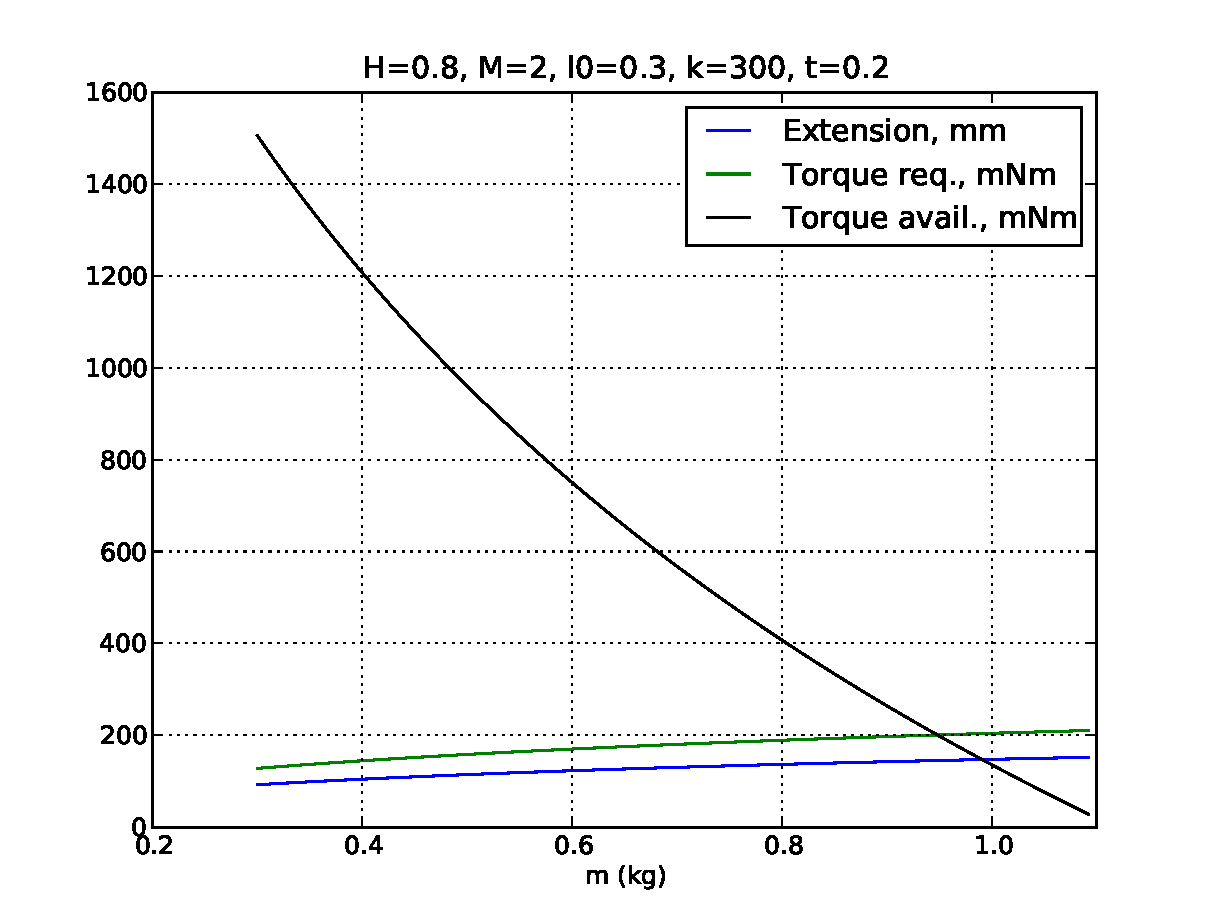
\includegraphics[scale=0.6]{fig/2mass_m.pdf}
\caption{Torque variation with m}
\label{fig:3_torque2mass}
\end{figure}

Fig. \ref{fig:3_torque2mass} shows the required torque  for extending springs to compensate the energy 
lost during impact fully within 0.2 sec. It is observed that m is the single most important parameter in 
hopper design. The required torque is a very strong function of the leg mass. As this mass increases, we 
need a larger motor to satisfy torque requirements. It is noted that a value of about 0.4--0.6 kg
can be called a reasonable estimate for the leg mass as we can easily choose a motor delivering the 
required torque for these values.\\

It is also seen that an extension of about 11 cms with a single spring of k = 300 Nm is needed to 
compensate the energy loss for hopping heights of 80 cms. So we should ensure that we can provide a 
maximum extension around 15 cms.

\subsection*{Impact Analysis}
The desired hopping height dictates a hopping frequency. Intuitively, smaller hopping height results in 
large number of impacts per time and consequently in larger energy loss per unit time. This is seen from 
Fig. \ref{fig:3_freq_height} because the hopping frequency is closer to the natural frequency for small 
hopping heights. However, beyond this consideration, since the hopper is a spring mass system, it 
possesses a natural frequency of its own. If the hopping frequency is near to this natural frequency, a 
large amount of energy is taken away by impact forces in every cycle. We intend to arrive at a range of 
values for the masses to ensure a large difference between the hopping frequency ($\omega_{hop}$) and the 
natural frequency ($\omega_{nat}$).
\begin{figure}[!h]
\centering
\subfloat[Freq. variation with height]{\label{fig:3_freq_height}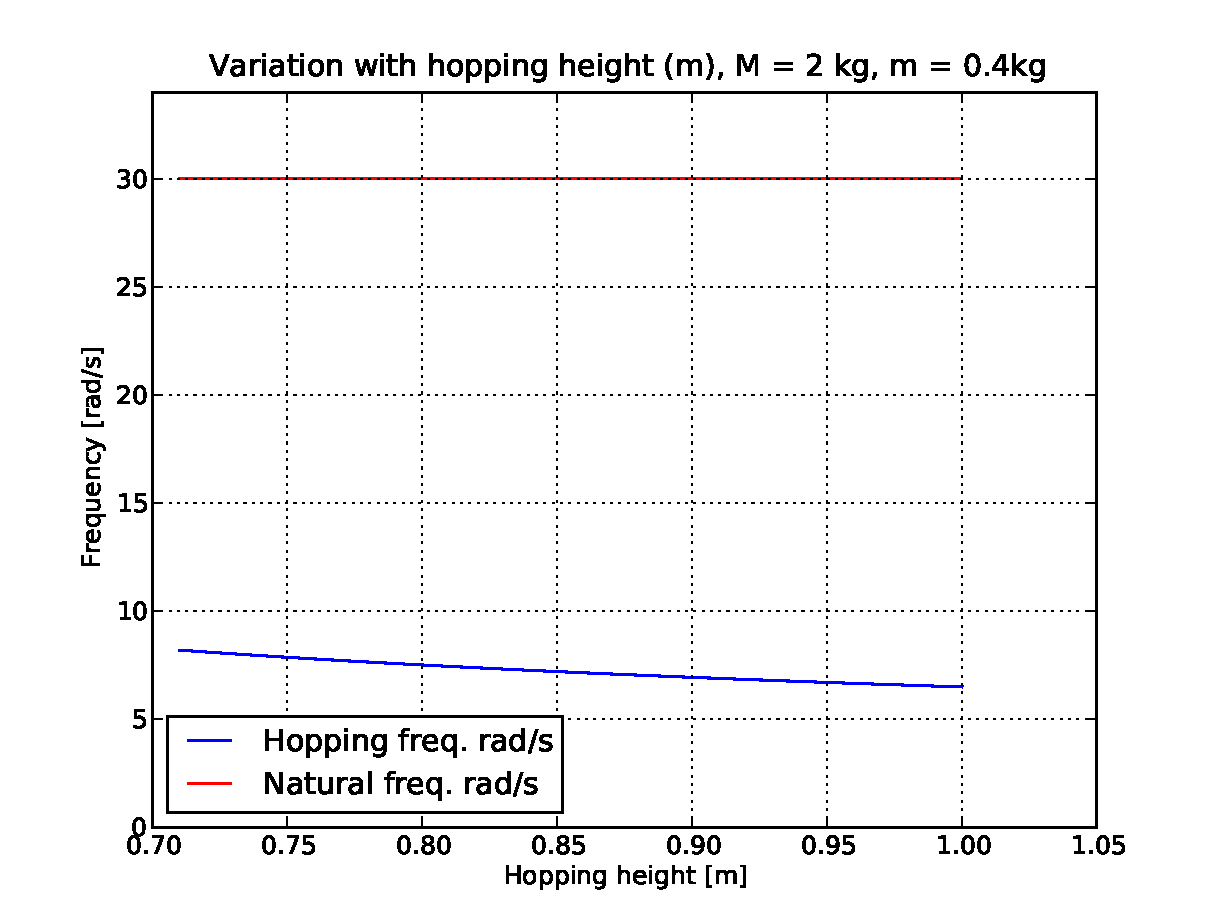
\includegraphics[width=0.5\textwidth]{fig/freq_hopheight.pdf}}
\subfloat[Freq. variation with m]{\label{fig:3_freq_m}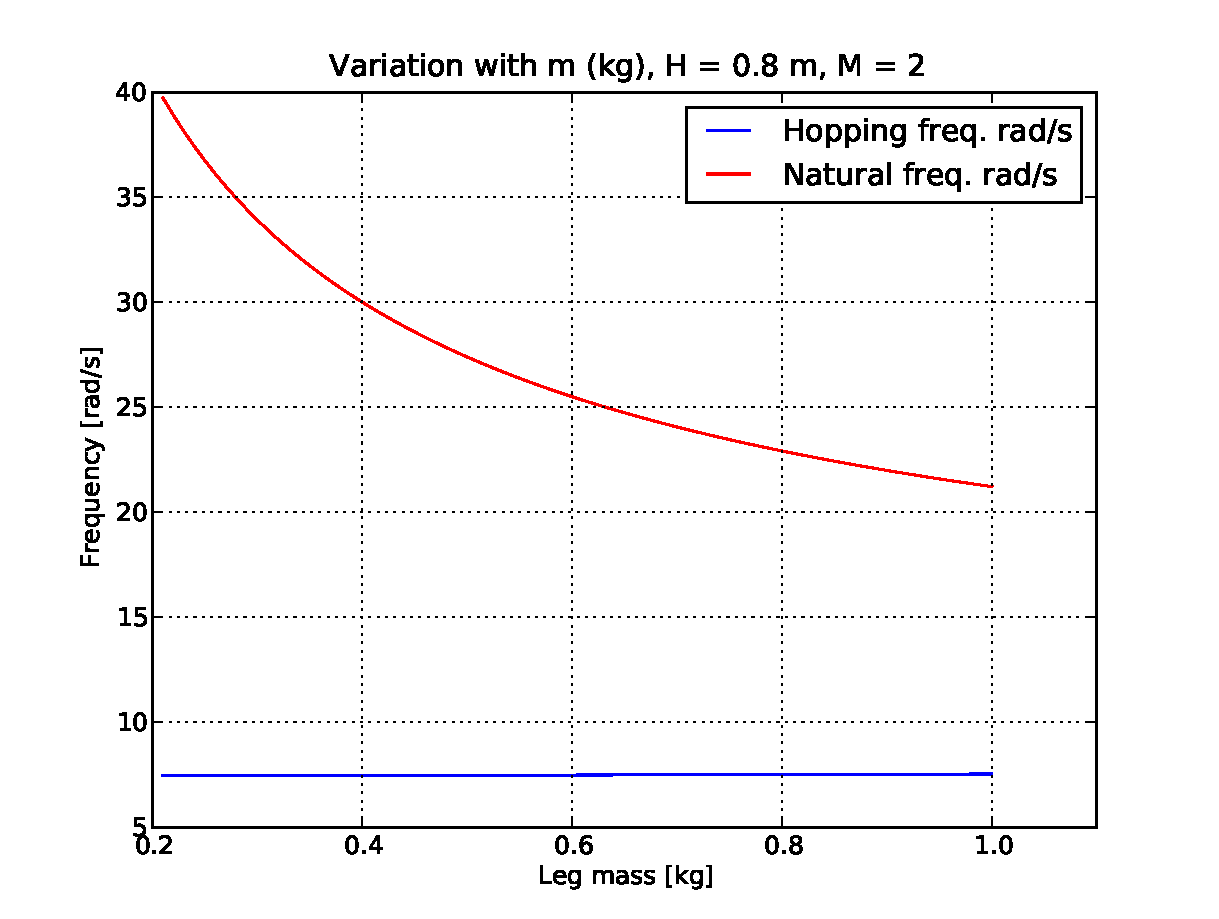
\includegraphics[width=0.5\textwidth]{fig/freq_m.pdf}}
\caption{Impact Analysis : Frequency variation}
\label{fig:4_freq_var}
\end{figure}
Fig. \ref{fig:3_freq_m} succinctly depicts all the above analysis. As the leg mass increases, the hopping frequency goes closer to the natural frequency i.e. more impact per unit time. To compound matters, more and more energy is lost per impact. So the conclusion from impact analysis is that the leg mass should be as low as possible. It is also seen from Fig. \ref{fig:3_freq_m} that \mbox{m = 0.4 -- 0.6 kg} is a good solution as well as an achievable one. 

\subsection*{Reaction Wheel}
For achieving a running gait with the hopper, it has to be started with the exact initial pitch and 
horizontal velocity. For any other initial condition, the hopper is pitch unstable and will not be able to 
continue the running gait. As mentioned in \cite{shanmug}, an offset mass acts as a passive stabilization 
to the pitch attitude of the hopper. To get rid of this need for exact initial condition which is quite 
impractical, we design a reaction wheel on the hopper. This will result in torque coupling on the pitch 
axis and thus provide an active control over the pitch of the robot.\\

We consider the case where the pitch is such that we have no horizontal velocity and no stabilization impulse from the ground. This pitch is reoriented to 30 degrees within one hop which corresponds to a huge horizontal velocity of 13.5 m/s. The stable pitch will be less than this for lower velocities. In actual operation
there will be large reaction wheel torques only while converting the initial condition into a stable
running gait. After that there will only be small control torques about the stable pitch angle.
\begin{figure}[!h]
\centering
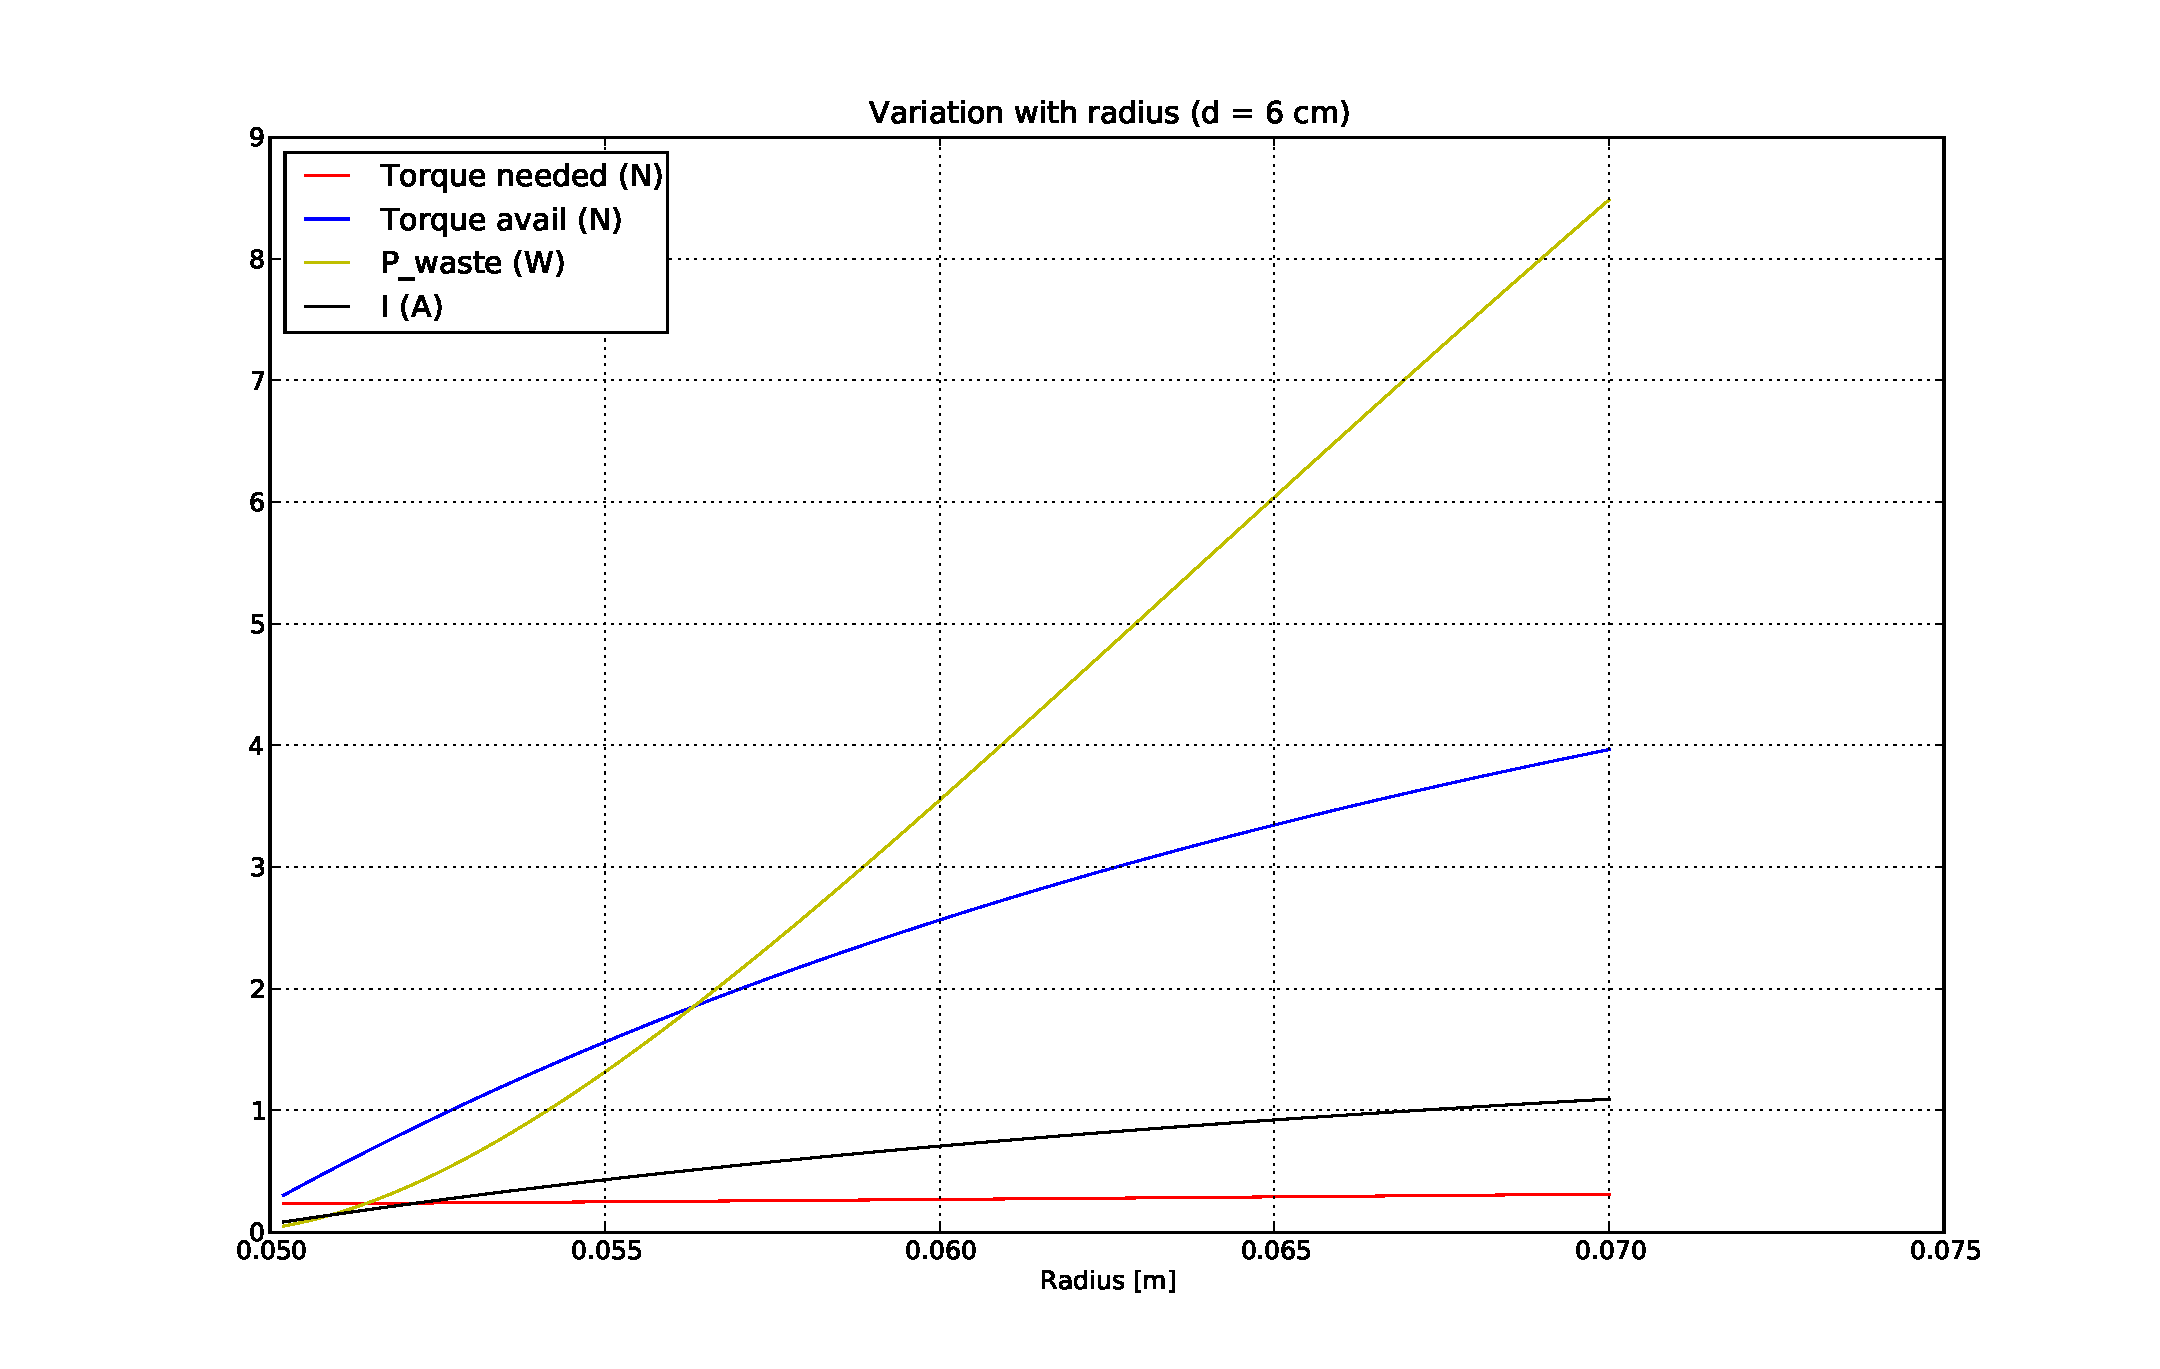
\includegraphics[scale=0.4]{fig/rewac_radius.pdf}
\caption{Torque requirements vs radius}
\label{fig:3_rewac_torque}
\end{figure}
Figs. \ref{fig:3_rewac_torque} has been plotted for distance of C.G. = 6 cms and radius of the reaction wheel taken as 6 cm (mass = 1.5 kg) after a similar analysis for variation in CG. We can see that the required torque for reorientation as mentioned in above is around 500 mNm with output power being around 1.5 W.

\section{Components}
\subsection*{Motors}
\begin{description}
 \item[\textsf{Reaction wheel motor}]
  3257CR024 motor is chosen with a standard gear box of 14.4 : 1. The stall current is below 5A and can be easily handled with the motor drivers designed using MOSFETs with 512 cpr encoders.
  \item[\textsf{Spring extension motor}]
  We take common values of worm-worm wheel diamter ratio (0.5), pressure angle (20 deg), helix angle for 
  worm (25 deg) and co-efficient of friction $\mu = 0.3$. The torque required from the motor is not more 
  than 200 mNm. The total power required for this task is about 4.5 W. We choose the 2342CR024 motor 
  for this task. The gear box is taken as a 43 : 1 with 512 cpr encoders.
  \item[\textsf{Servo 3003}]
  This is used for the ratchet and paul mechanism as well as the motor sleeve disengagement. The torque requirements are satisfied easily since not much torque is needed.
  \item[\textsf{Motor Driver}]
  The stall current of both the motors is near 5A and hence a conventional readymade H-bridge will not work. I designed a H-bridge using MOSFETs (CSD 16404) and MOSFET drivers (TPS 2836) to provide good drive to the motors with a maximum current of 21A and $R_{GS} =$ 4.1 $\Omega$. It can be controlled using just two microcontroller pins.
  \begin{figure}[H]
  \centering
  \subfloat[Top side]{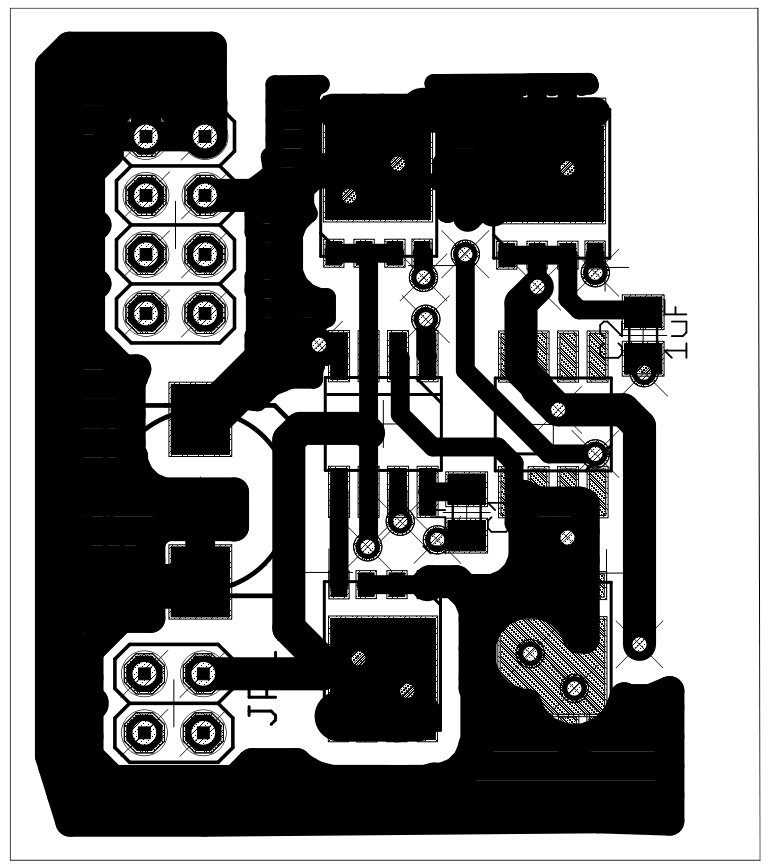
\includegraphics[width=0.35\textwidth, angle=90]{fig/hbridge_top.png}}
  \subfloat[Bottom side]{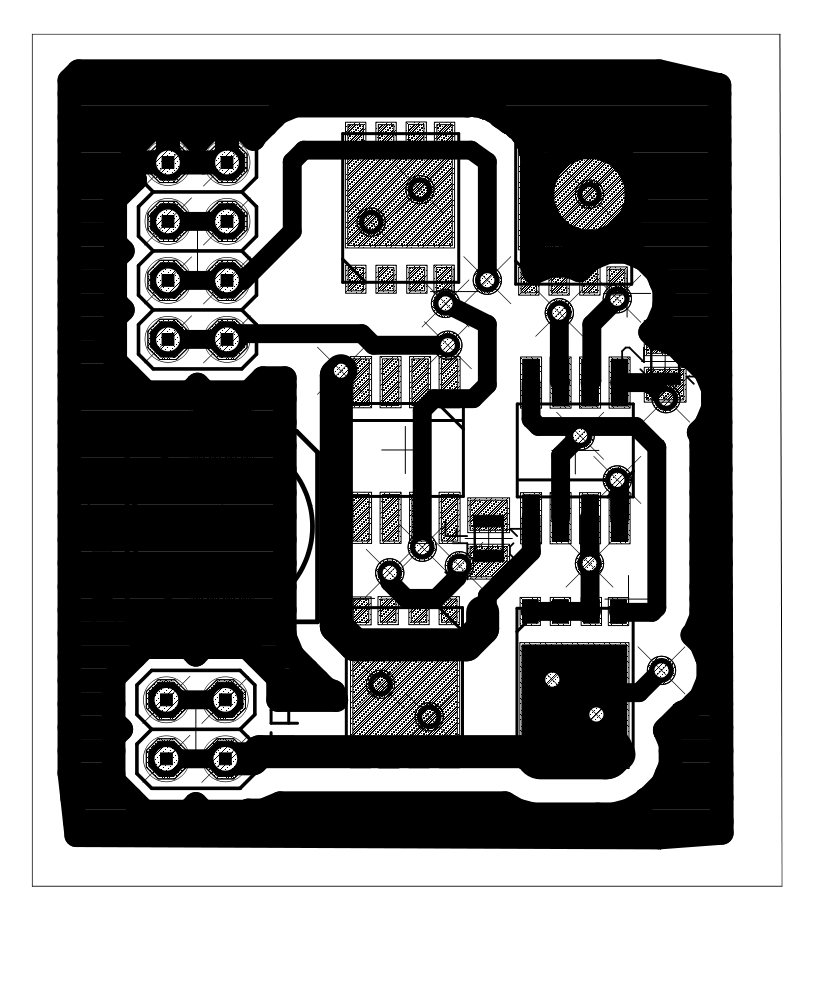
\includegraphics[width=0.35\textwidth, angle=90]{fig/hbridge_bot.png}}
  \caption{MOSFET Hbridge}
  \label{fig:3_hbridge}
  \end{figure}
  \end{description}

\subsection*{Inertial Measurement Unit}
\begin{description}
  \item[\textsf{Accelerometer - ADIS 16201}]
  Provides 14-bit signed readings. The accelerometer has a sensitivity of 2.162 LSB/mg with a noise of 22 
  LSB. The accelerometer also consists of an inclinometer to measure the angle with respect to the ground. 
  However, it provides a sensitivity of only 10 LSB/deg. This necessitates the need of onboard inverse 
  tangent tables to get the pitch angle from accelerometer readings. The bandwidth of the accelerometer is 
  2.25 KHz.
  \item[\textsf{Single Axis Gyroscope - ADIS 16255}]
  Provides 14-bit signed readings with internal temperature calibration. The sensitivity of the gyroscope 
  is $0.07326$ $^o/$s/LSB for the whole range of $\pm\;320$ $^o/$s with a noise of $0.48$ $^o/$s.  The 
  bandwidth of the gyroscope is 50 Hz which severely limits the update rate of the filter.
\end{description}

\subsection*{Computing}
\begin{description}
  \item[\textsf{Microcontroller}]
  Microchip dsPIC33F64MC804 can run at 40 MIPS with an onboard flash memory of
  64 KB along with a 16 KB SRAM. There are a host of integrated peripherals like Serial Peripheral 
  Interface (SPI), UART, Analog to Digital converter (ADC), Quadrature Encoder (QEI) and timers to 
  generate Pulse Width Modulation (PWM) that can be used for motor control. Pickit 2 is the USB programmer 
  used to program the flash of the microcontroller.
  \item[\textsf{XBee Modules}]
  Used to provide a wireless link between the embedded system and the PC with the help of a custom made 
  FT232 USB-UART converter. This is a major tool for all debugging and grabbing telemetry.
  \begin{figure}[H]
  \centering
  \subfloat[Top Side]{\label{fig:3_brddoctop}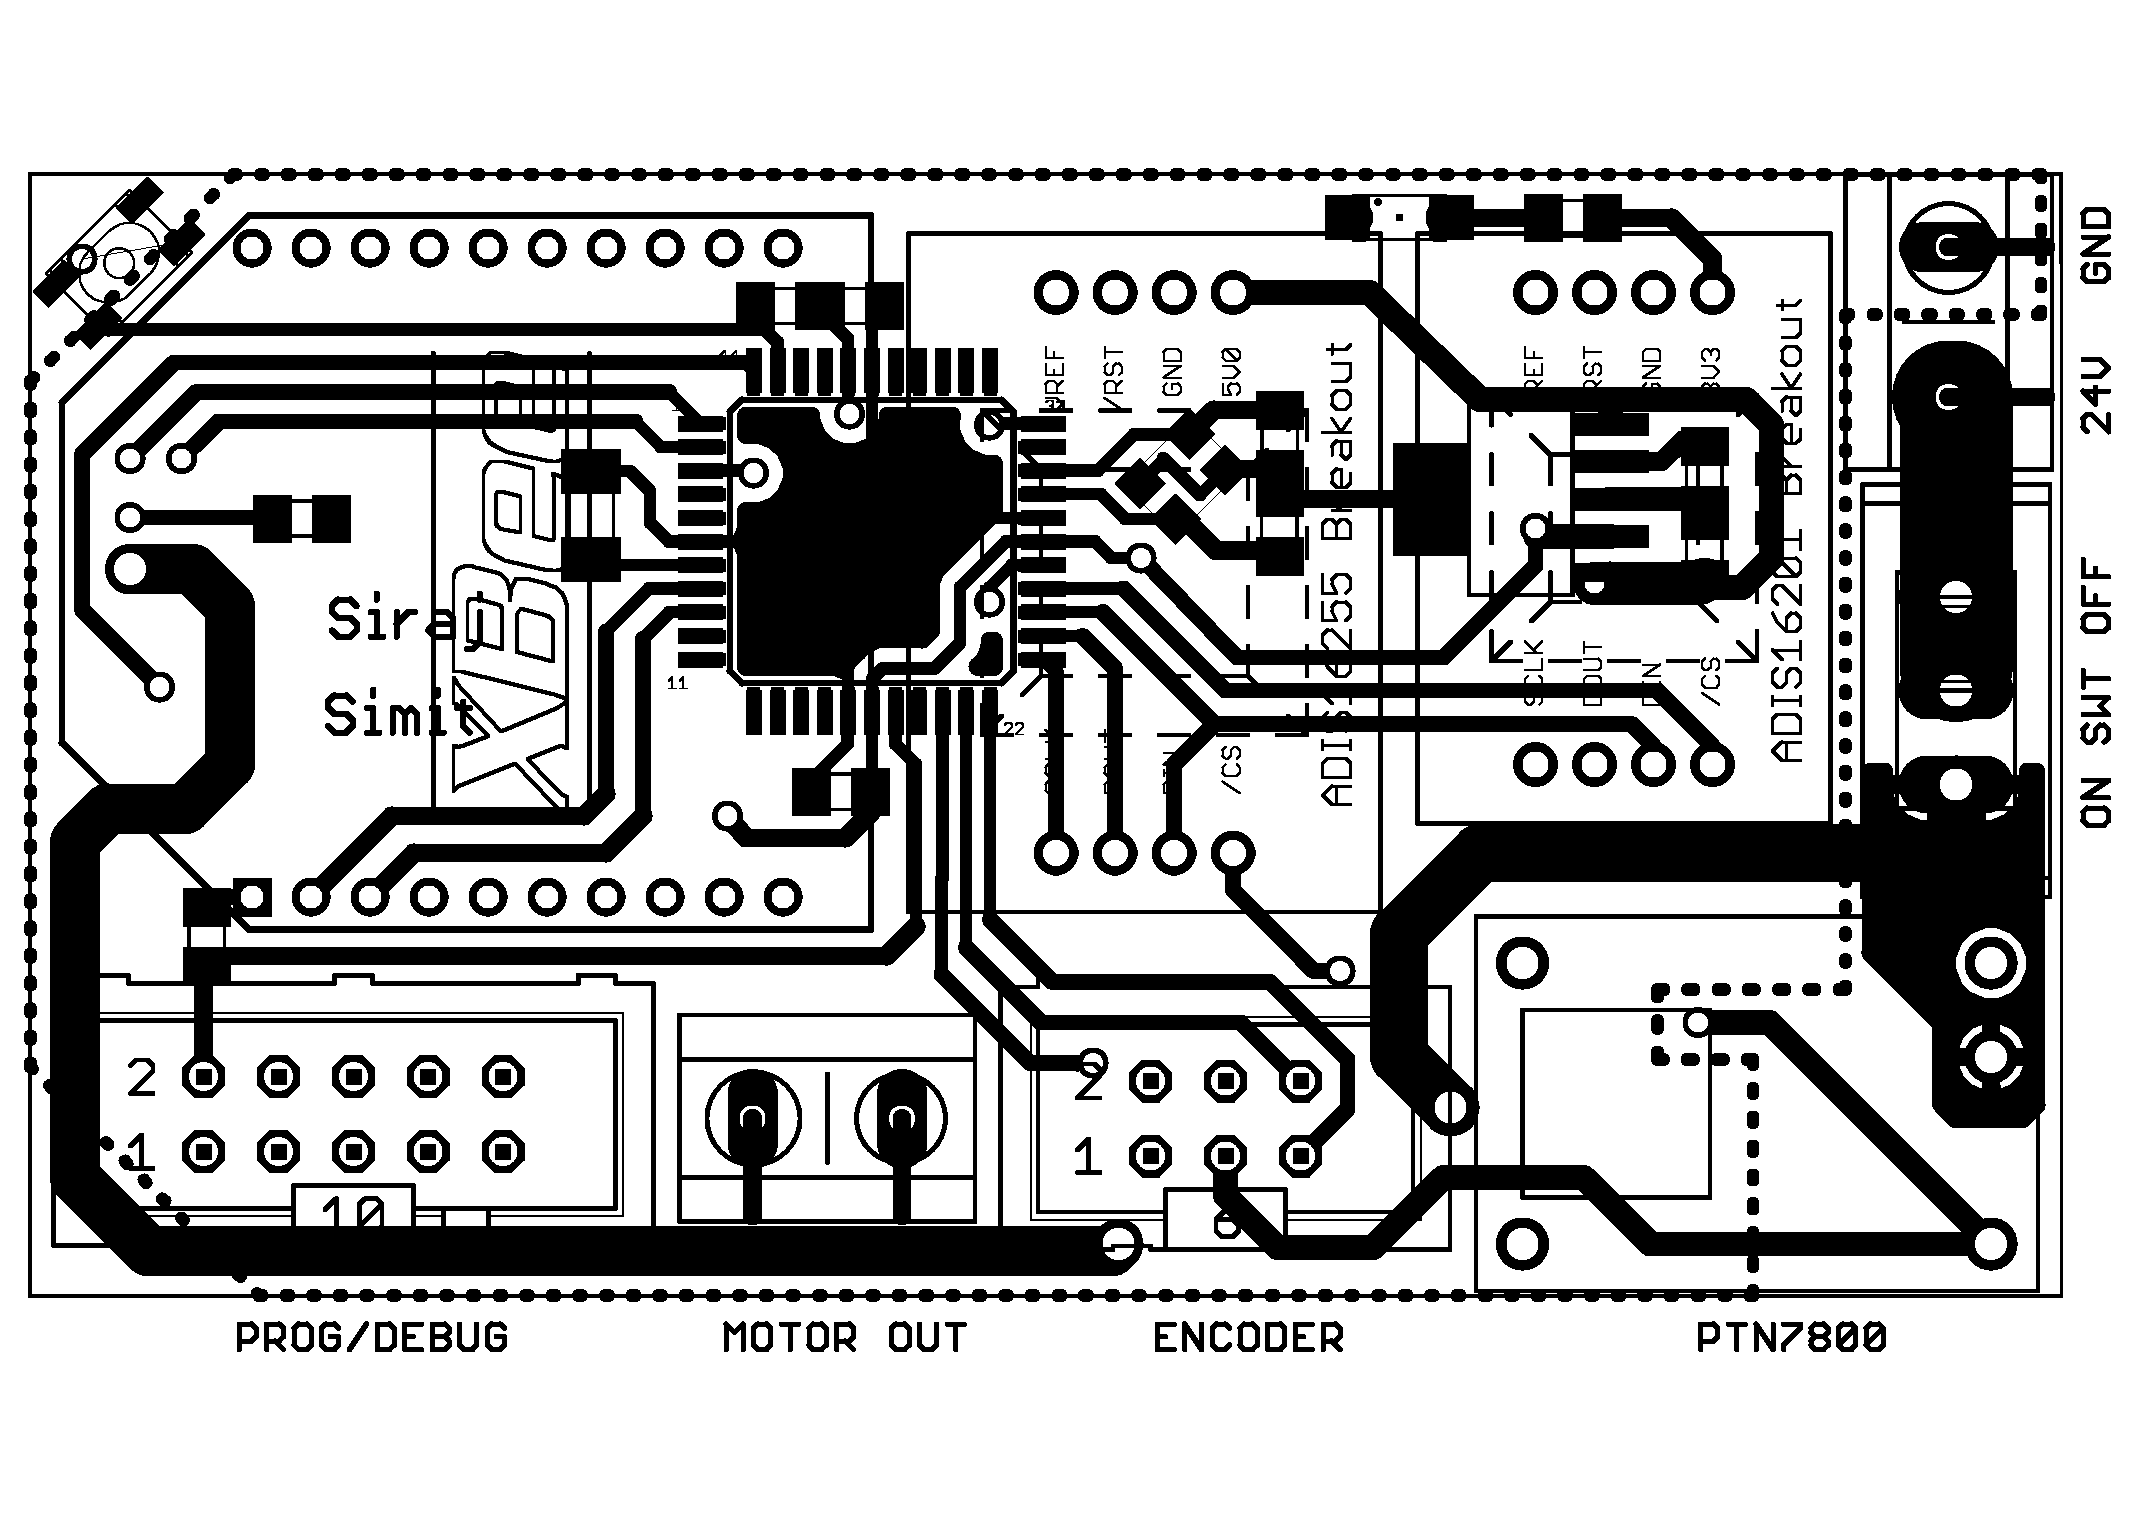
\includegraphics[width=0.49\textwidth]{fig/rewac_top.pdf}}
  \subfloat[Bottom Side]{\label{fig:3_brddocbot}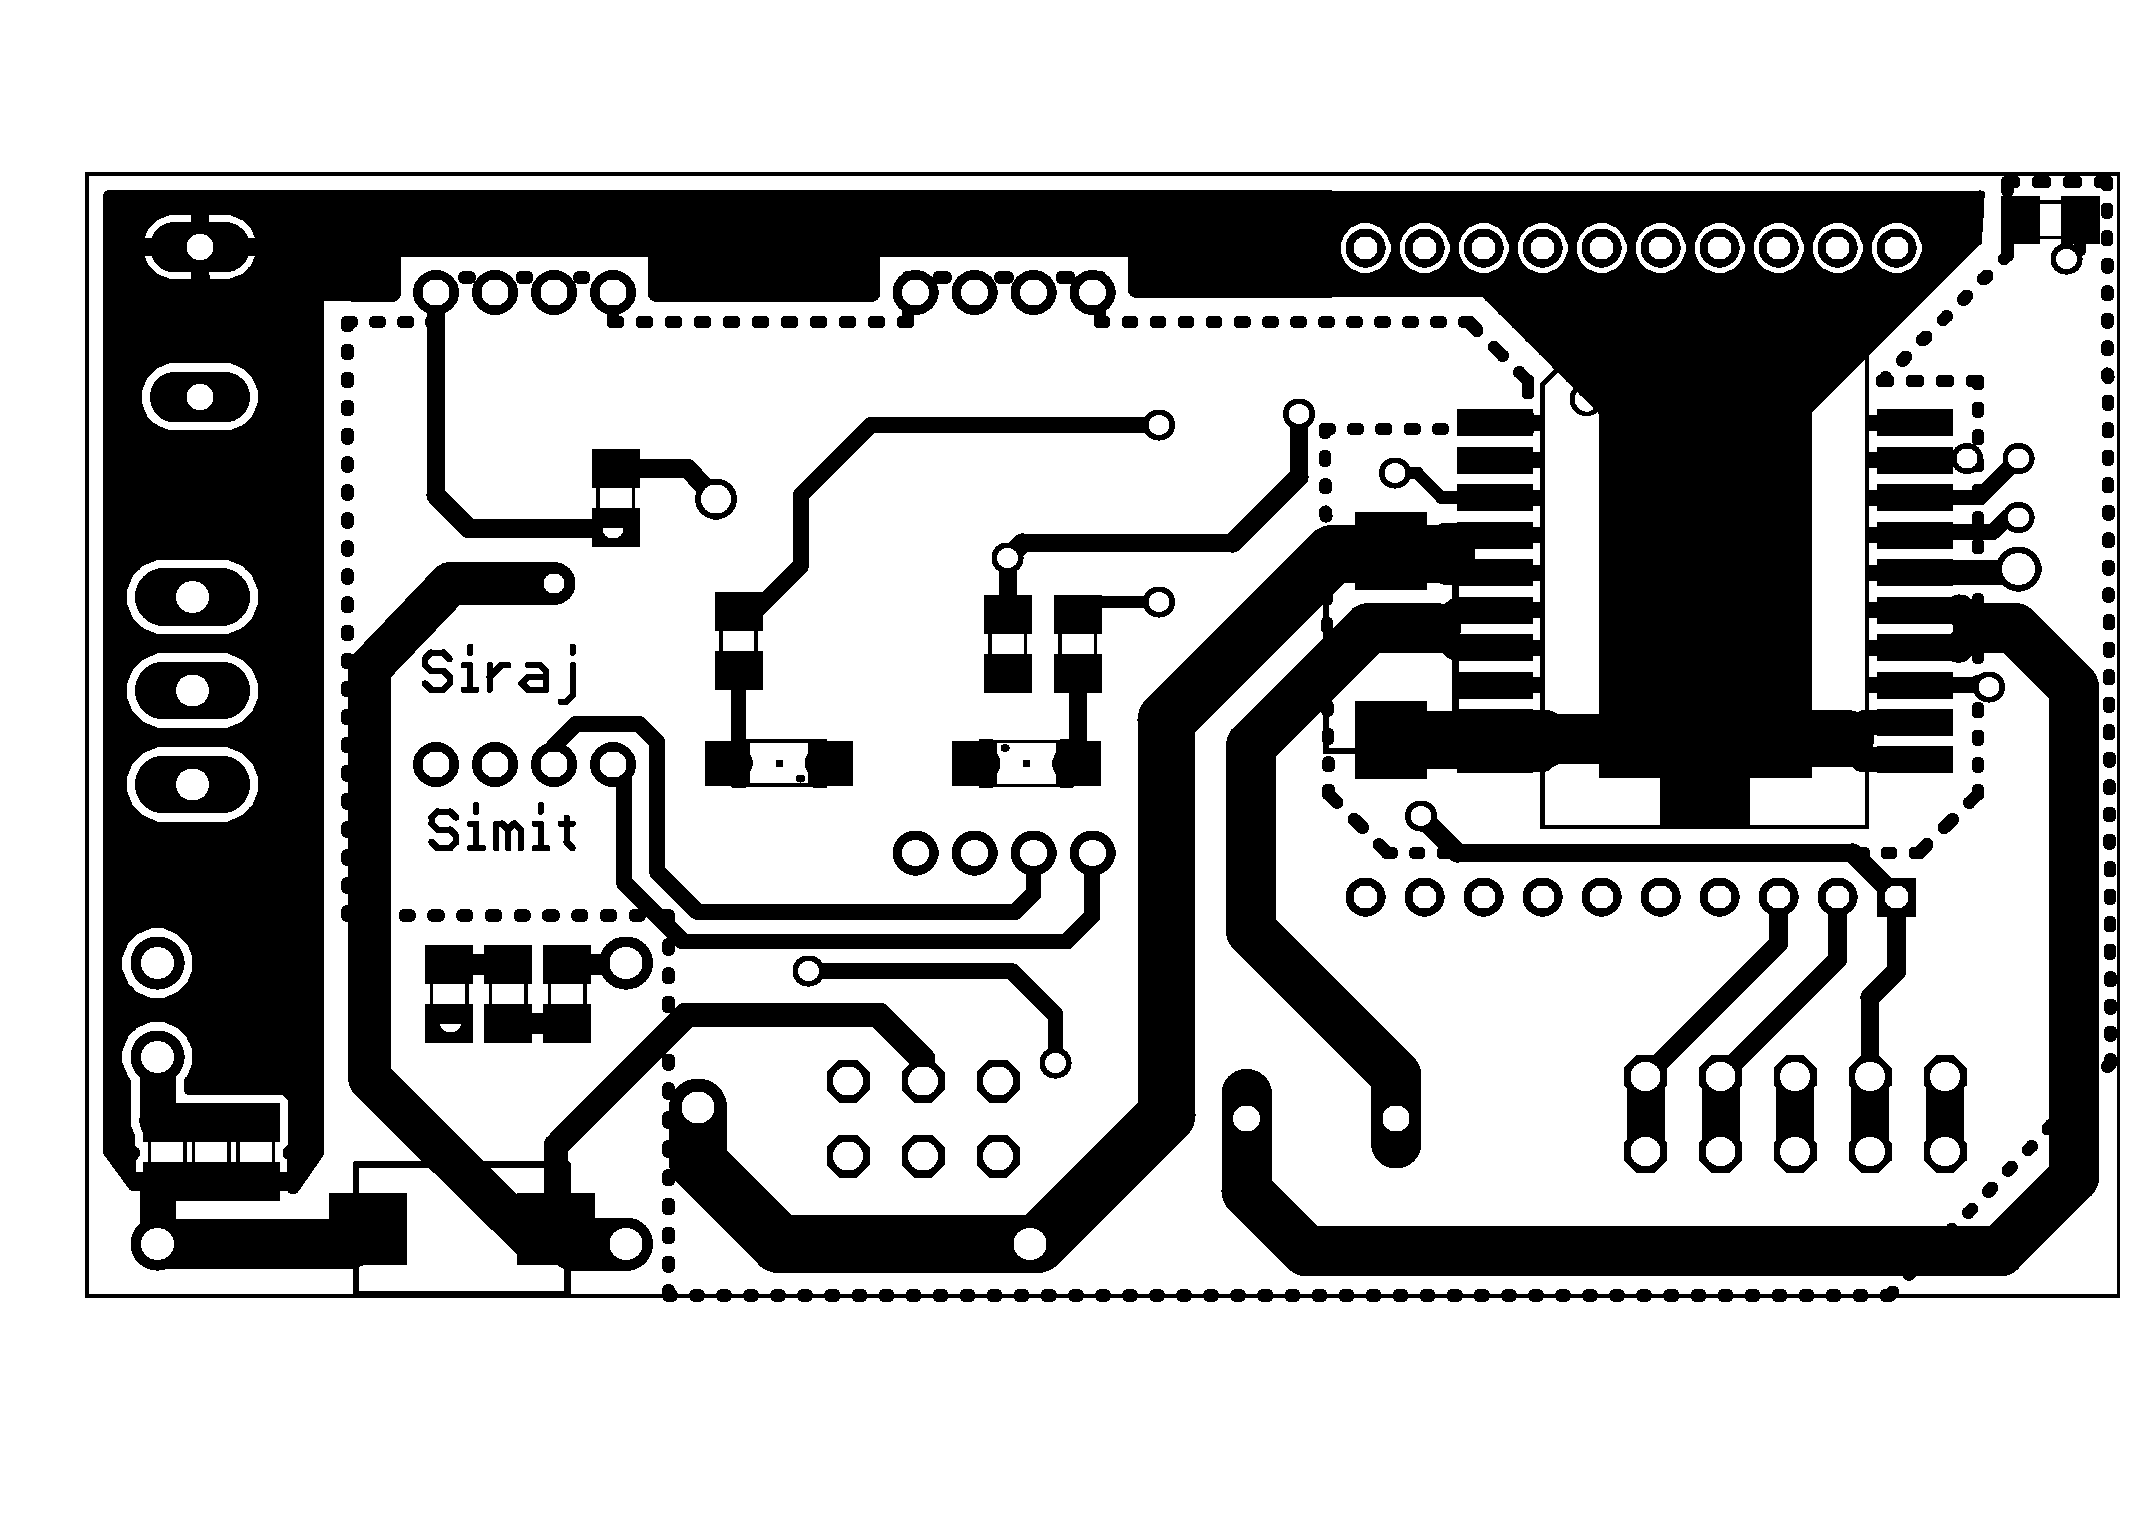
\includegraphics[width=0.49\textwidth]{fig/rewac_bot.pdf}}
  \caption{On-board controller pinouts}
  \label{fig:brddoc}
  \end{figure}
\end{description}
Fig. \ref{fig:3_brddocbot} and \ref{fig:3_brddoctop} show the onboard controller that was used for the experiements. A new board incorporating all drives and motors has been designed but not fabricated yet.












